% !TEX TS-program = xelatex
\documentclass[aspectratio=169,11pt,professionalfonts]{beamer}

% Theme
\usetheme[numbering=fraction,progressbar=frametitle]{metropolis}
\metroset{block=fill}

% Fonts (XeLaTeX/LuaLaTeX)
\usepackage{fontspec}

% Language & basic packages (mathtools MUST come before unicode-math)
\usepackage[english]{babel}
\usepackage{graphicx}
\usepackage{booktabs}
\usepackage{tabularx}
\usepackage{amsmath,amssymb,mathtools}
\usepackage{xcolor}
\usepackage{csquotes}

% Unicode-math must be loaded AFTER mathtools
\usepackage{unicode-math}
% Main text font per user request
\setmainfont{Fira Code}
\setmonofont{Fira Code}
% Math font for formulas (Fira Code has no math)
\setmathfont{latinmodern-math.otf}

% Graphics search paths (relative to this file)
\graphicspath{{../../pro-default-model/results/}{../../paper/Long_term/}}

% Macros
\newcommand{\E}{\mathbb{E}}
\newcommand{\bbP}{\mathbb{P}}
\newcommand{\Y}{\mathcal{Y}}
\newcommand{\1}{\mathbb{1}}
\DeclareMathOperator{\Lsig}{L}

% Title
\title{Default with Policy\,–\,Randomness Overestimation (PRO)}
\subtitle{Pivoted Pricing, Deleveraging, and a Stability Illusion}
\author{Chen Gao}
\institute{National School of Development, Peking University}
\date{October 15}

% Section page
\setbeamertemplate{section page}{\centering\begin{minipage}{0.9\linewidth}\centering\usebeamerfont{section title}\insertsection\par\end{minipage}}
\AtBeginSection{
  {\setbeamertemplate{footline}{}
  \begin{frame}[plain]\sectionpage\end{frame}}
}

\begin{document}

% Title
\begin{frame}[plain]
  \titlepage
\end{frame}

% Agenda
\begin{frame}{Roadmap}
  \tableofcontents
\end{frame}

% Motivation
\section{Motivation}

\begin{frame}{A Persistent Puzzle}
  \begin{itemize}
    \item Some sovereigns face persistently high spreads despite moderate debt and
          improving fundamentals.
    \item Event evidence (e.g., Argentina’s inflation misreporting) shows spread
          decoupling beyond direct balance-sheet effects.
    \item Standard models struggle to match elevated average premia with lower
          volatility.
    \item This paper: a single pricing operator with a second-moment belief wedge (PRO)
          that \emph{pivots} price/spread schedules.
  \end{itemize}
\end{frame}

\begin{frame}{Argentina: Data Misreporting and Spread Decoupling}
  \begin{columns}[T,onlytextwidth]
    \column{0.5\textwidth}
    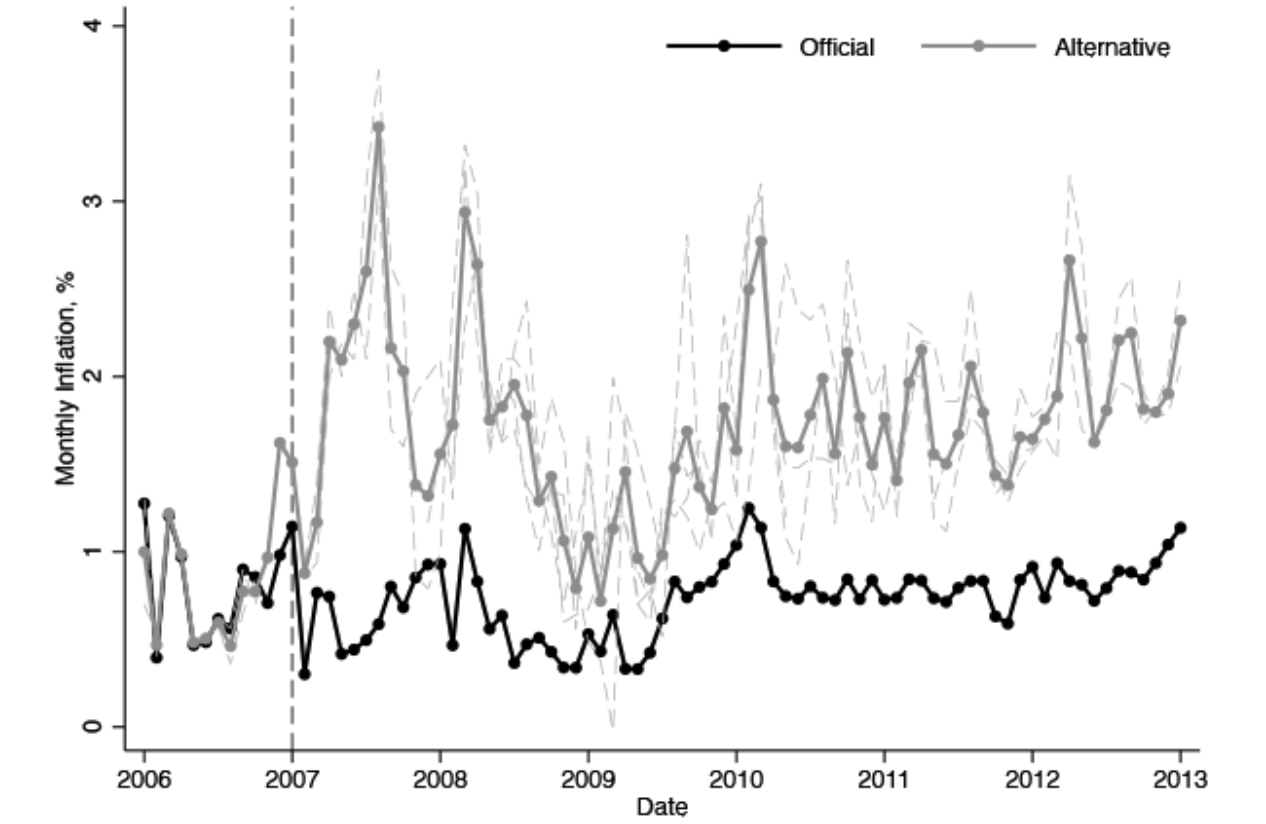
\includegraphics[width=\linewidth]{../../pro-default-model/results/inflation_arg.png}
    \vspace{0.3em}
    {\scriptsize Official CPI vs. alternative measures}
    \column{0.5\textwidth}
    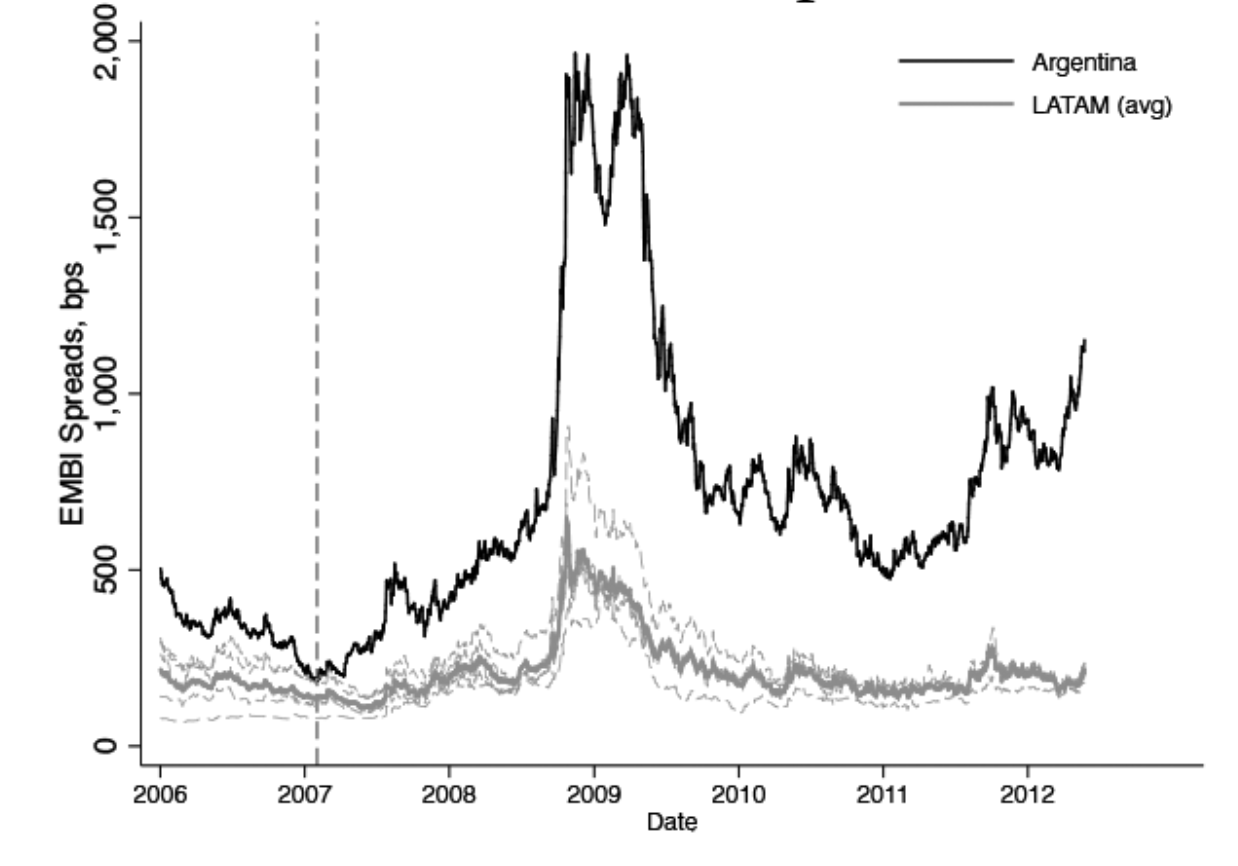
\includegraphics[width=\linewidth]{../../pro-default-model/results/spread_arg.png}
    \vspace{0.3em}
    {\scriptsize EMBI+ spreads: Argentina vs. LA peers}
  \end{columns}
  \vspace{0.3em}
  \begin{itemize}
    \item \textbf{Interpretation}: reputational channel (type) + \textbf{PRO} (policy dispersion) both active.
  \end{itemize}
\end{frame}

% Model
\section{Model}

\begin{frame}{Environment}
  \begin{itemize}
    \item \textbf{Endowment}: $\ln y'=(1-\rho_y)\mu_y+\rho_y\ln y+\sigma_y\varepsilon'$, $\varepsilon'\sim\mathcal N(0,1)$.
    \item \textbf{Debt}: long-term bond with coupon $\kappa$, decay $\delta$, risk-free rate $r$.
    \item \textbf{Default}: exclusion prob. $1-\gamma$; cost $h(y)=y-\max\{0,\lambda_0 y+\lambda_1 y^2\}$.
    \item \textbf{Preferences}: $u(c)=(c^{1-\sigma}-1)/(1-\sigma)$, discount $\beta$.
  \end{itemize}
\end{frame}

\begin{frame}{Discrete Choice: Default and Borrowing}
  \textbf{Taste shocks (Gumbel)} yield smooth aggregator and logit rules.
  \begin{gather*}
    \textbf{Ex-ante value:}\quad V(y,B)=\eta\,\ln\!\Big( e^{V^D(y)/\eta}+e^{V^R(y,B)/\eta}\Big),\\
    \textbf{Default prob.:}\quad \bbP\{d{=}1\mid y,B\}=\Lsig\!\Big(-\tfrac{\Delta V(y,B)}{\eta}\Big)=\tfrac{e^{V^D/\eta}}{e^{V^D/\eta}+e^{V^R/\eta}},\\
    \textbf{Borrowing aggregator:}\quad V^R(y,B)=\rho\,\ln\!\sum_{B'\in\mathcal B} e^{W(y,B,B')/\rho},\\
    \textbf{Borrowing policy:}\quad \bbP\{B'\mid y,B\}=\frac{e^{W(y,B,B')/\rho}}{\sum_{\tilde B'} e^{W(y,B,\tilde B')/\rho}},
  \end{gather*}
  \vspace{-0.5em}
  where $\Delta V\equiv V^R{-}V^D$, $W(y,B,B')=u\big(y-\kappa B+[B'-(1{-}\delta)B]q(y,B')\big)+\beta\E V(y',B')$.
\end{frame}

\begin{frame}{Lenders and Pricing Operator}
  \textbf{PRO} scales the \emph{default logit} via tail weight $\symbf{\theta} \ge 1$:
  \begin{equation*}
    \boxed{\;P_{\theta}(y,B')=\Lsig\!\Big(-\tfrac{\Delta V(y,B')}{\theta\,\eta}\Big),\qquad \Lsig(z)=\tfrac{1}{1+e^{-z}}\;}
  \end{equation*}
  \textbf{Pricing operator (unique fixed point):}
  \begin{equation*}
    \boxed{\;(\mathcal T_{\theta} q)(B',y)=\tfrac{1}{1+r}\,\E_{y'|y}\!\Big[(1{-}P_{\theta}(y',B'))\big(\kappa+(1{-}\delta)\,\E_{B''|y',B'}q(y',B'')\big)\Big]\;}
  \end{equation*}
  \textbf{Slope (joint contraction) condition:}
  \begin{equation*}
    L_{Jq}L_{TV}\;<\;(1-\beta)\Big(1-\tfrac{1-\delta}{1+r}\Big)\quad\Rightarrow\quad \text{unique fixed point}.
  \end{equation*}
\end{frame}

% Pivot intuition
\section{Pivot Intuition}

\begin{frame}{One-Line Schematic of \textbf{Pivot}}
  \textbf{Compact schematic anchoring the single-crossing:}
  \begin{align*}
     & P_{\theta}(y,B')=\Lsig\!\Big(-\tfrac{\Delta V(y,B')}{\theta\eta}\Big),\quad \Delta V\equiv V^R{-}V^D,                                     \\
     & \Rightarrow\quad \mathrm{sign}\big( P_1{-}P_{\theta}\big)=-\,\mathrm{sign}(\Delta V),                                                     \\
     & \Rightarrow\quad \mathrm{sign}\big(q_{\theta}{-}q_1\big)=\mathrm{sign}\,\E[(P_1{-}P_{\theta})\Pi]\;=\;-\,\mathrm{sign}(\Delta V),\;\Pi>0.
  \end{align*}
  \textbf{Define the threshold} $B^*(y):\ \Delta V(y,B^*(y))=0$. Then:
  \begin{itemize}
    \item \textbf{$B' < B^*(y)$} (safe region, $\Delta V>0$): $\;q_{\theta}<q_1$ (\textbf{PRO premium}).
    \item \textbf{$B' > B^*(y)$} (near default, $\Delta V<0$): $\;q_{\theta}>q_1$ (\textbf{softened doom}).
  \end{itemize}
\end{frame}

\begin{frame}{Pivot: Proof Sketch and Comparative Statics}
  \textbf{Operator order}: If $P_{\theta}\gtrless P_1$ pointwise, positivity of payoff kernel implies $(\mathcal T_{\theta} q)\lessgtr (\mathcal T_1 q)$.
  \begin{itemize}
    \item \textbf{Sign}: $\mathrm{sign}(P_1-P_{\theta})=-\mathrm{sign}(\Delta V)$ $\Rightarrow$ single crossing at $\Delta V{=}0$.
    \item \textbf{Threshold monotonicity}: $B^*(y)$ increases in $y$ (rational schedule shifts out more than PRO).
    \item \textbf{Policies}: higher \textbf{default threshold}, \textbf{deleveraging}, \textbf{higher mean spreads}.
  \end{itemize}
\end{frame}

% Quantitative
\section{Quantitative Results}

\begin{frame}{Calibration (Quarterly, EM stylized)}
  \begin{itemize}
    \item Preferences and endowment: $\sigma=2$, $\beta=0.9775$, $\rho_y=0.95$,
          $\sigma_y=0.005$.
    \item Debt: $\delta=0.04$ (5y duration), $\kappa=\delta{+}r$, $r=1\%$/qtr,
          $\gamma=0.125$.
    \item Default cost: $h(y)=y-\max\{0,\lambda_0 y+\lambda_1 y^2\}$ with
          $(\lambda_0,\lambda_1)=(-0.48,0.525)$.
    \item Taste shocks small: $\eta=5\times10^{-4}$, $\rho=10^{-5}$; grids: $N_y{=}201$,
          $N_B{=}600$.
    \item Scenarios: $\theta\in\{1,10,100\}$.
  \end{itemize}
\end{frame}

\begin{frame}{Business Cycle Moments}
  \begin{columns}[T,onlytextwidth]
    \column{0.56\textwidth}
    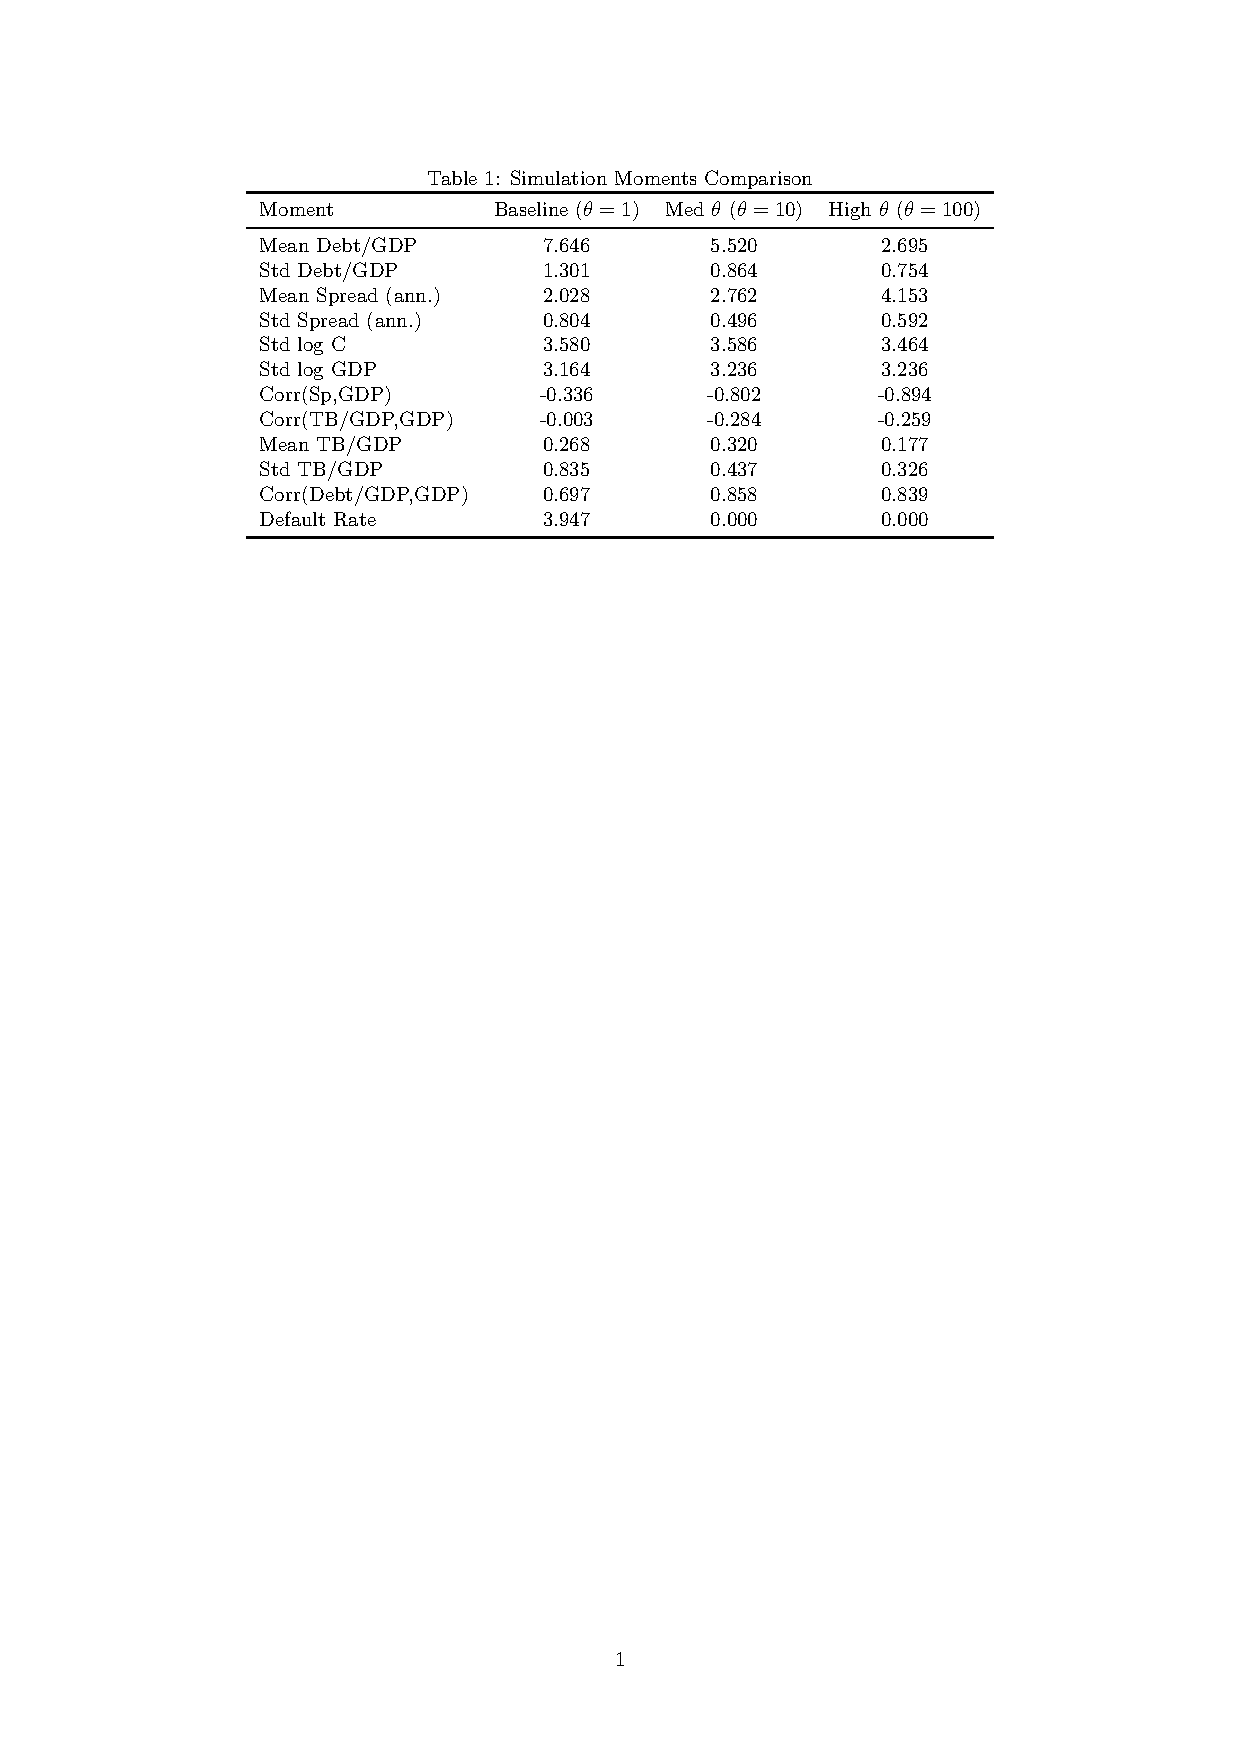
\includegraphics[width=\linewidth]{../../pro-default-model/results/moments_comparison_table.pdf}
    \column{0.44\textwidth}
    \begin{itemize}
      \item \textbf{Higher avg spreads} with \textbf{deleveraging} (pivot wedge dominates composition).
      \item Spreads \textbf{more countercyclical}; volatility of spreads/debt
            \textbf{falls} (\textbf{stability illusion}).
      \item Consumption volatility \textbf{nearly unchanged}; risk insurance
            \textbf{impaired}.
    \end{itemize}
  \end{columns}
\end{frame}

\begin{frame}{Price, Spread, and Default Risk}
  \begin{columns}[T,onlytextwidth]
    \column{0.33\textwidth}
    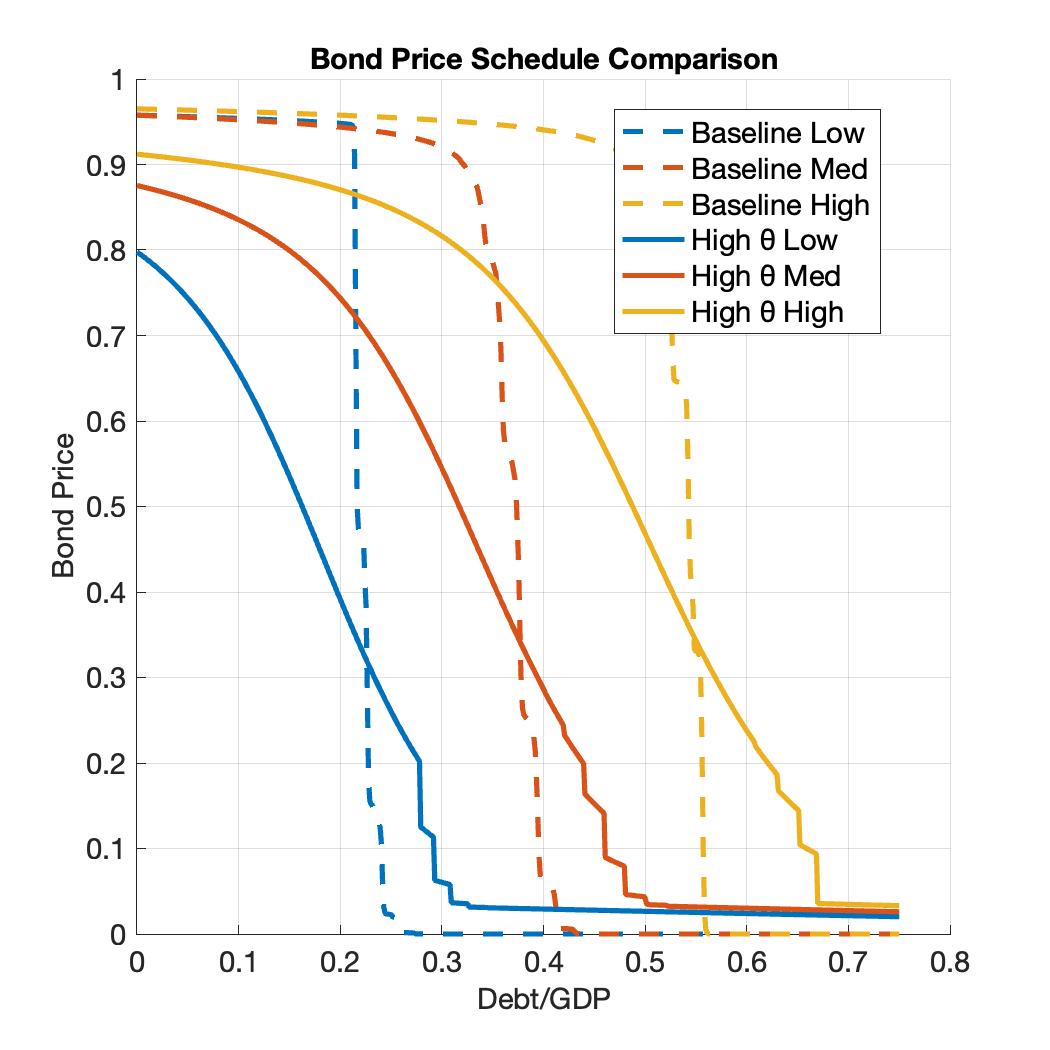
\includegraphics[width=\linewidth]{../../pro-default-model/results/bond_price_comparison.png}\\[0.3em]
    {\scriptsize Bond prices}
    \column{0.33\textwidth}
    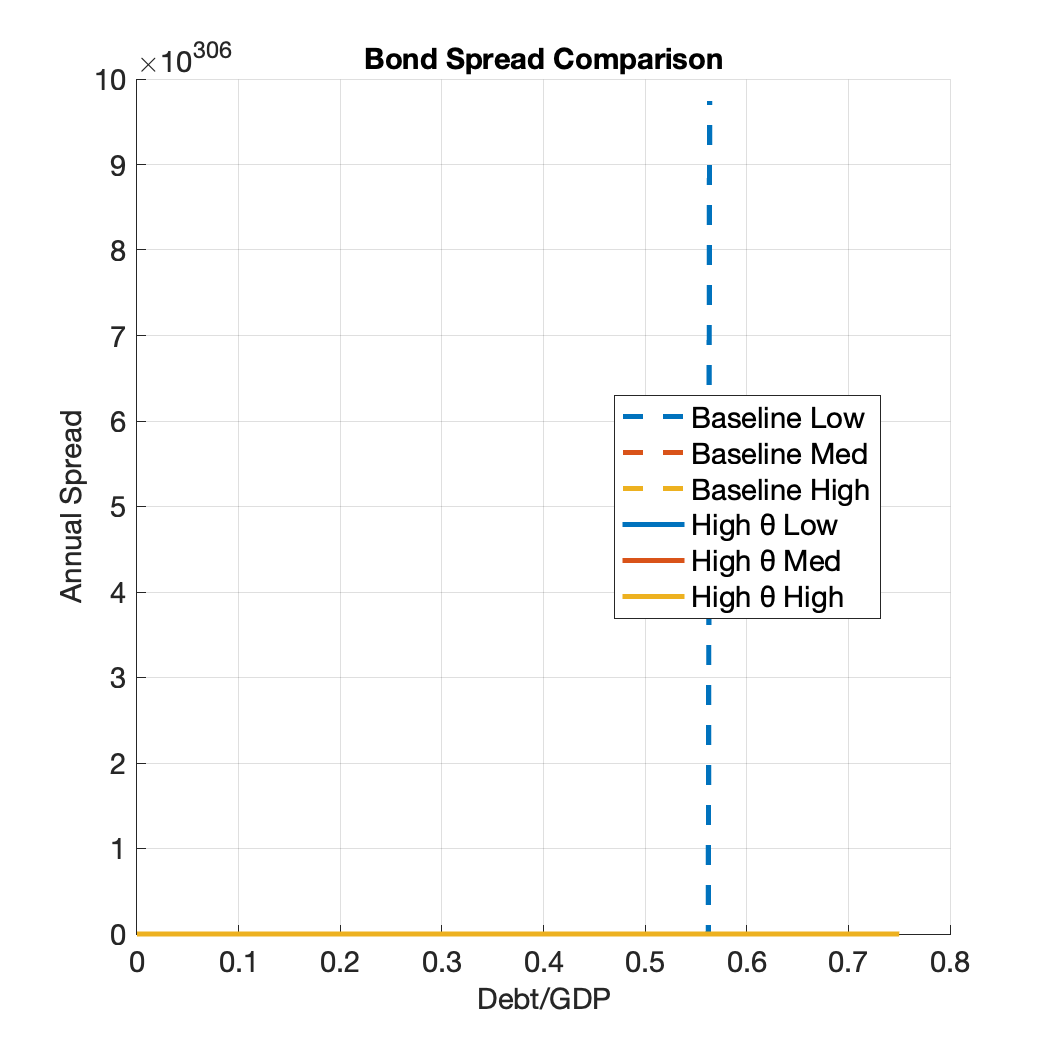
\includegraphics[width=\linewidth]{../../pro-default-model/results/spread_comparison.png}\\[0.3em]
    {\scriptsize Spreads}
    \column{0.33\textwidth}
    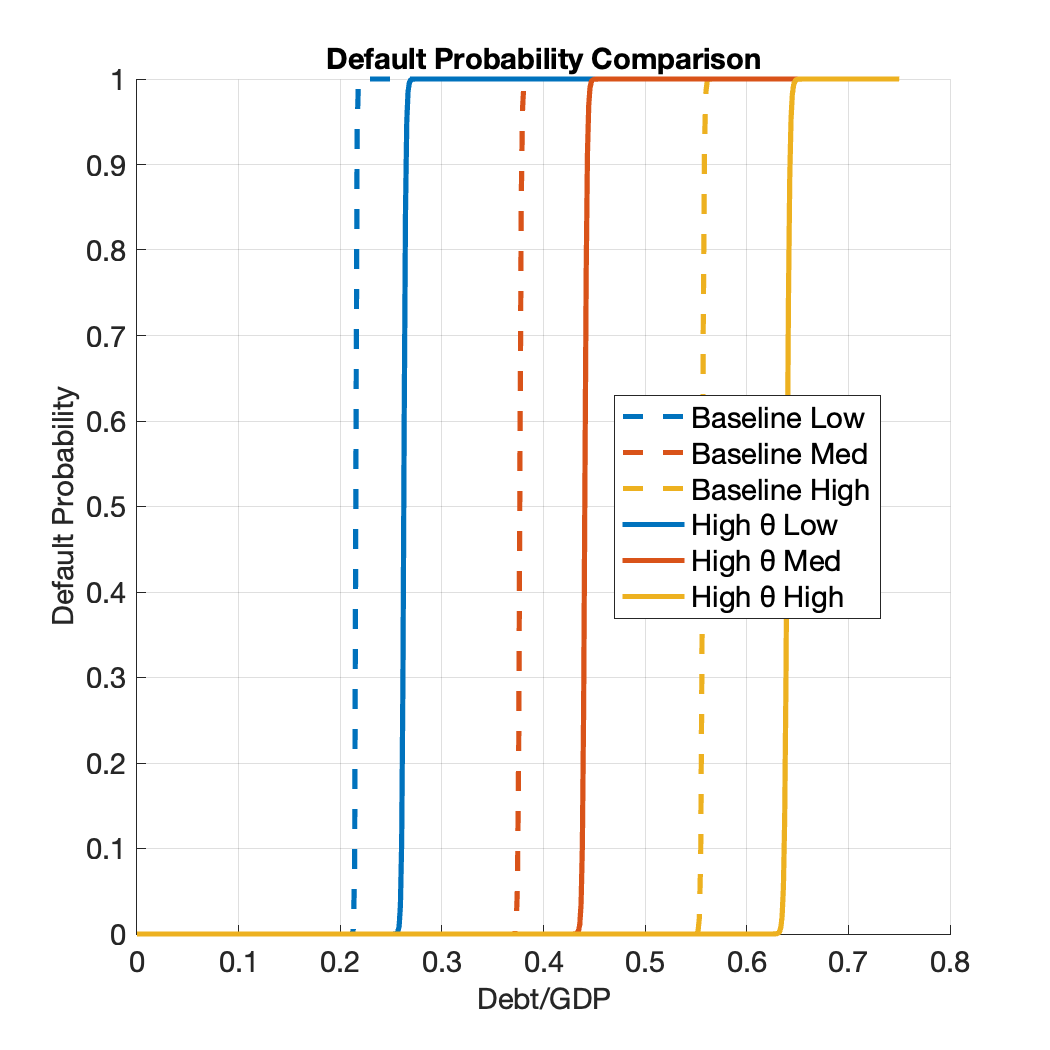
\includegraphics[width=\linewidth]{../../pro-default-model/results/default_prob_comparison.png}\\[0.3em]
    {\scriptsize Default probabilities}
  \end{columns}
  \vspace{0.3em}
  {\scriptsize \textbf{Single-crossing pivot} around $B^*(y)$; PRO discounts \textbf{safe region} and \textbf{softens near-doom}.}
\end{frame}

\begin{frame}{Impulse Responses: Transitory Shock}
  \begin{columns}[T,onlytextwidth]
    \column{0.5\textwidth}
    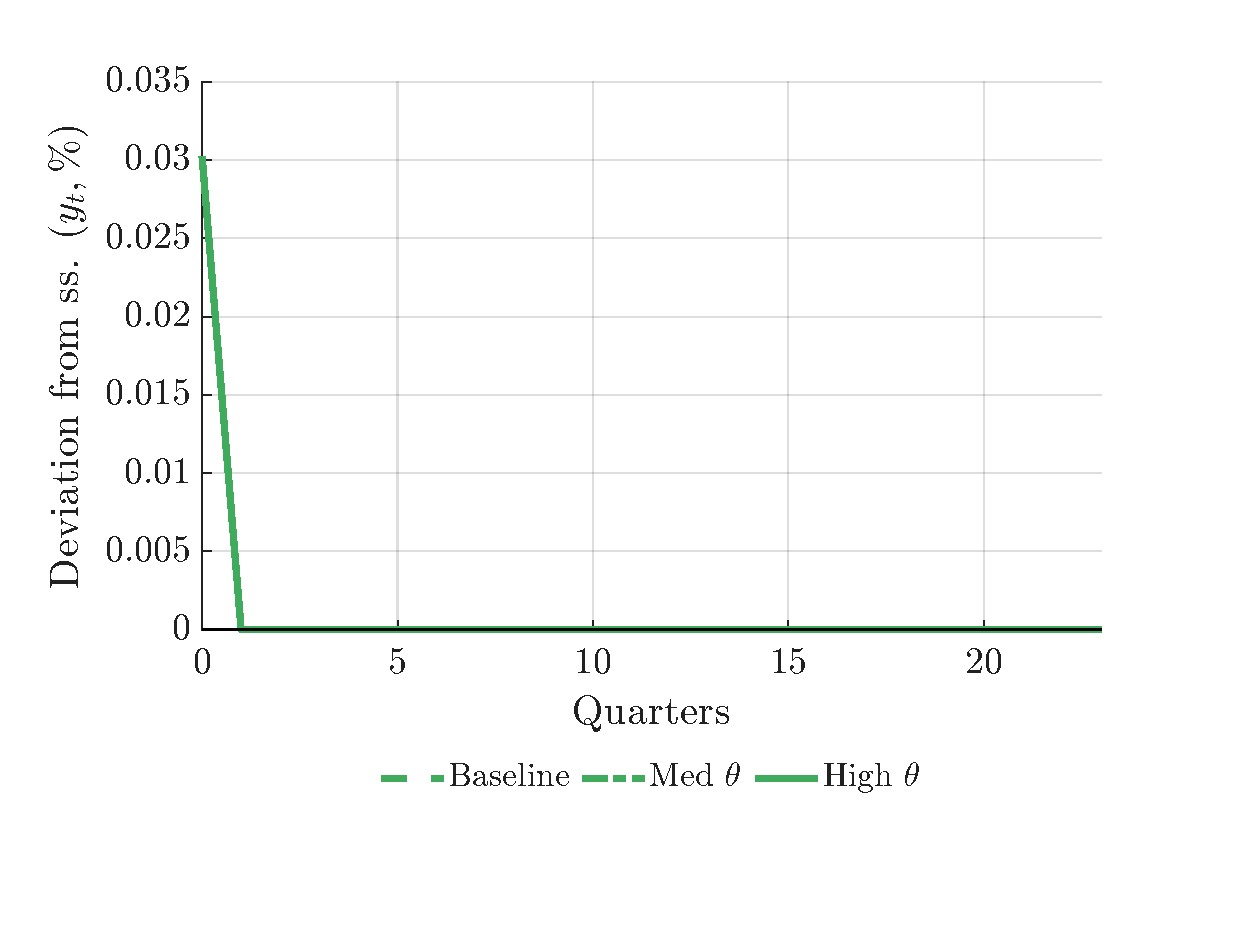
\includegraphics[width=\linewidth]{../../pro-default-model/results/comparison_figure_13.pdf}\\[-0.5em]
    {\scriptsize Output}
    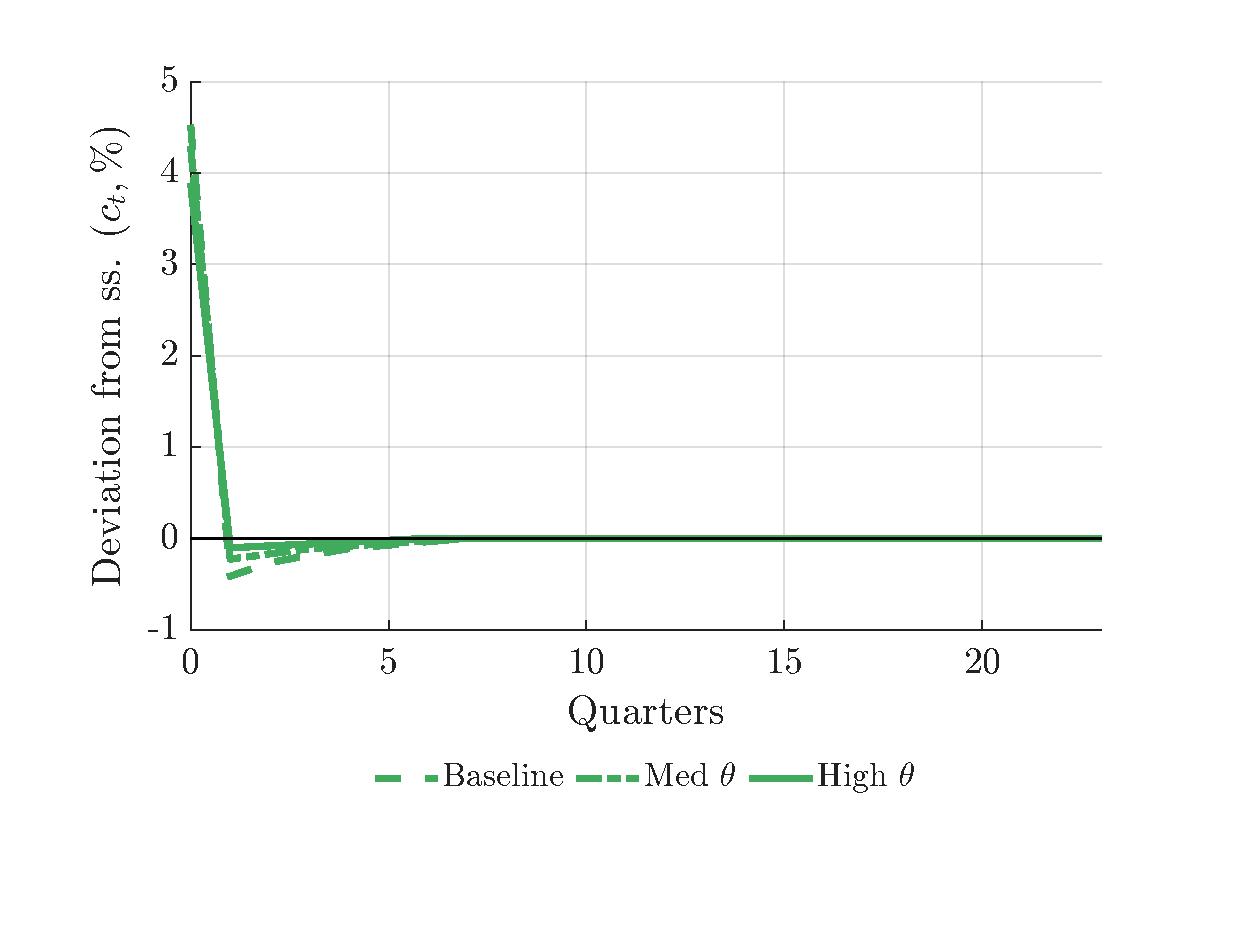
\includegraphics[width=\linewidth]{../../pro-default-model/results/comparison_figure_15.pdf}\\[-0.5em]
    {\scriptsize Consumption}
    \column{0.5\textwidth}
    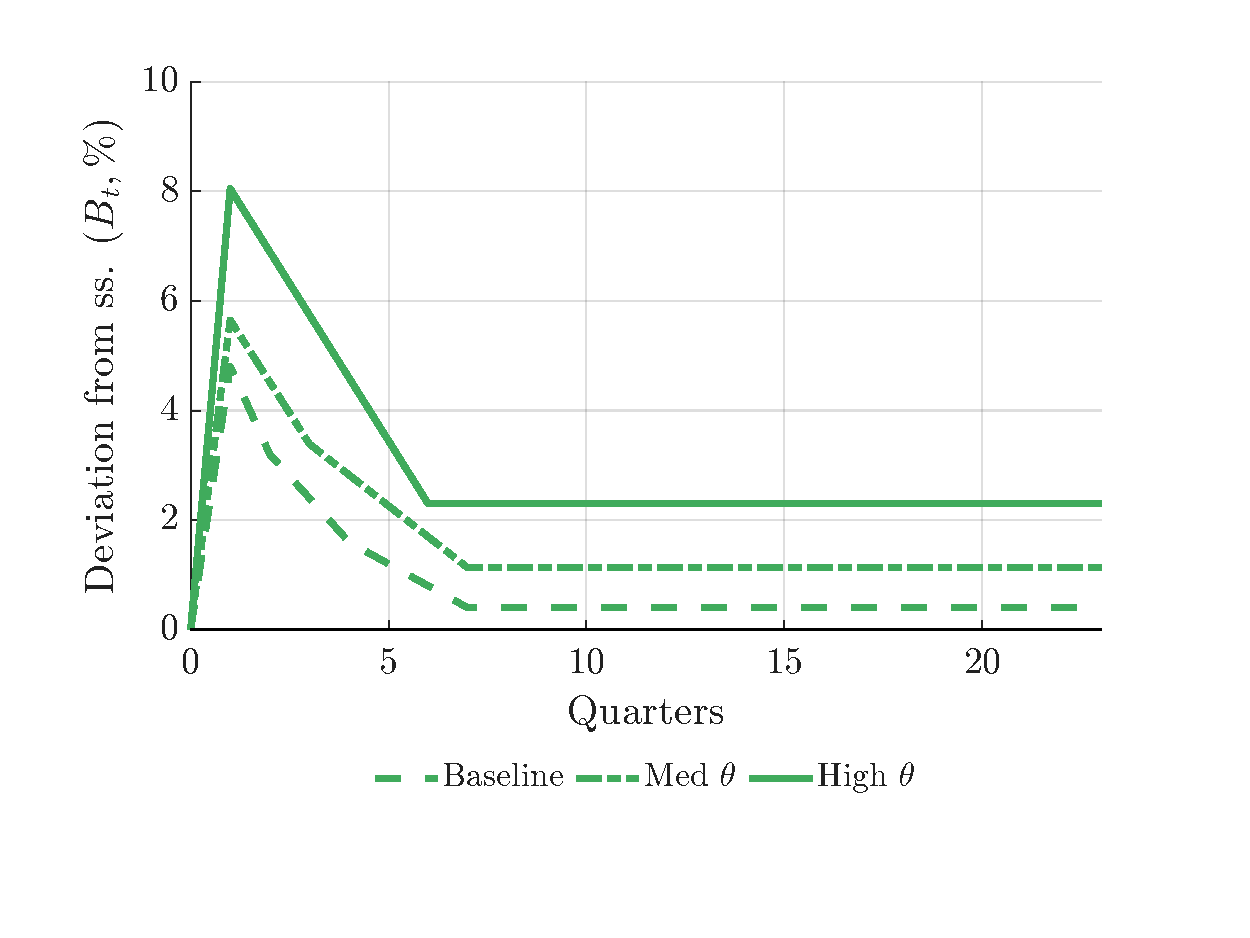
\includegraphics[width=\linewidth]{../../pro-default-model/results/comparison_figure_14.pdf}\\[-0.5em]
    {\scriptsize Debt}
    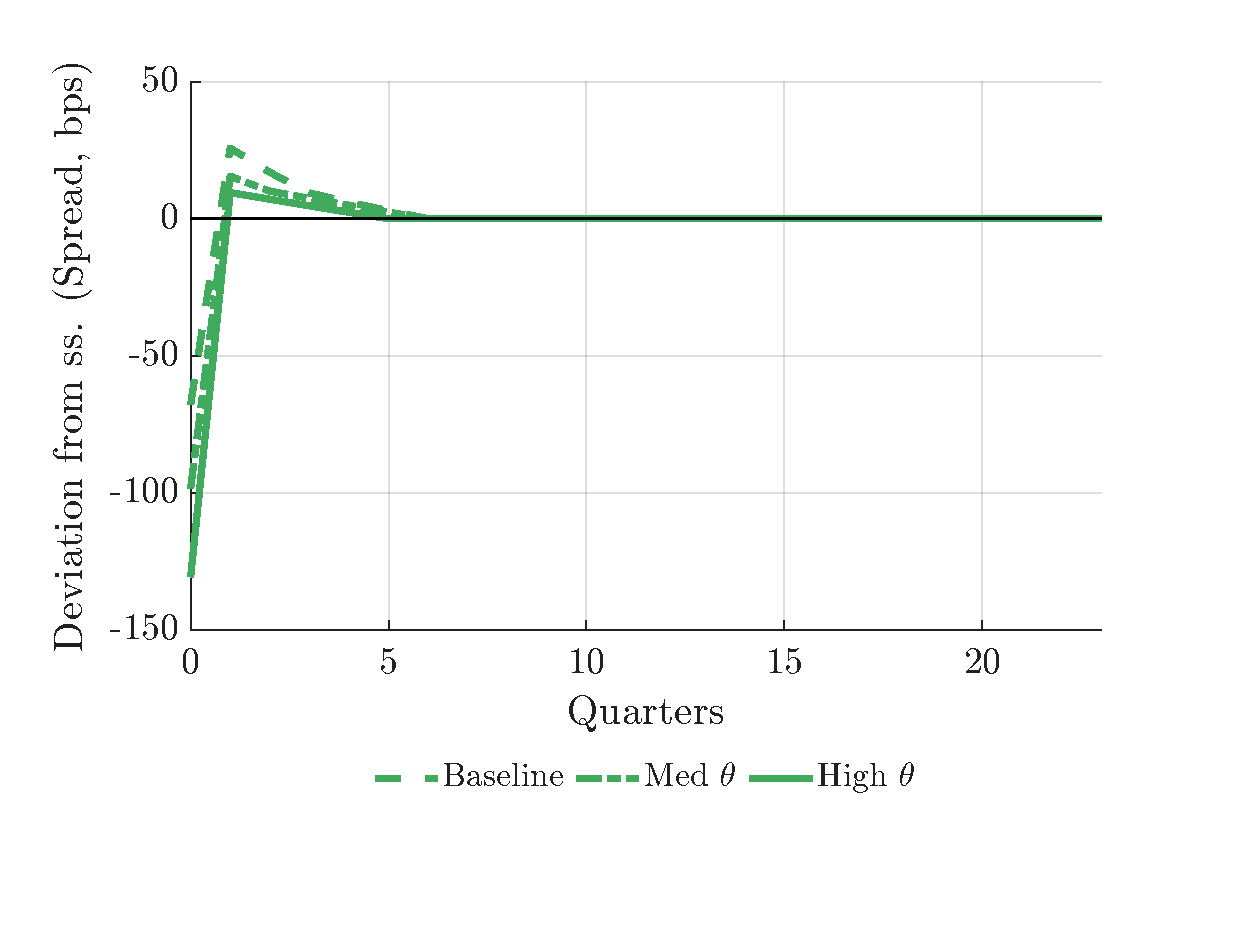
\includegraphics[width=\linewidth]{../../pro-default-model/results/comparison_figure_16.pdf}\\[-0.5em]
    {\scriptsize Spread}
  \end{columns}
\end{frame}

\begin{frame}{Impulse Responses: Persistent Shock}
  \begin{columns}[T,onlytextwidth]
    \column{0.5\textwidth}
    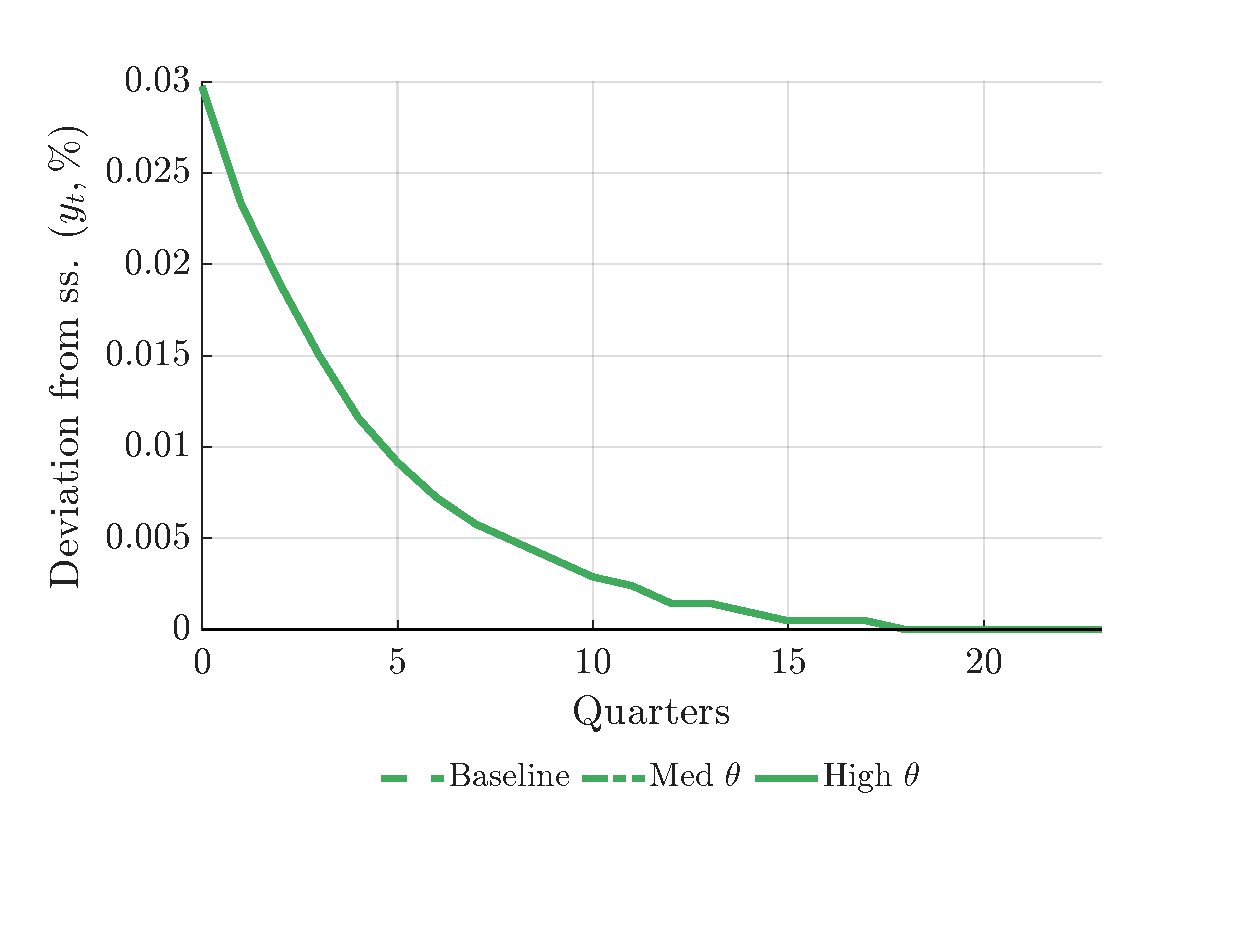
\includegraphics[width=\linewidth]{../../pro-default-model/results/comparison_figure_17.pdf}\\[-0.5em]
    {\scriptsize Output}
    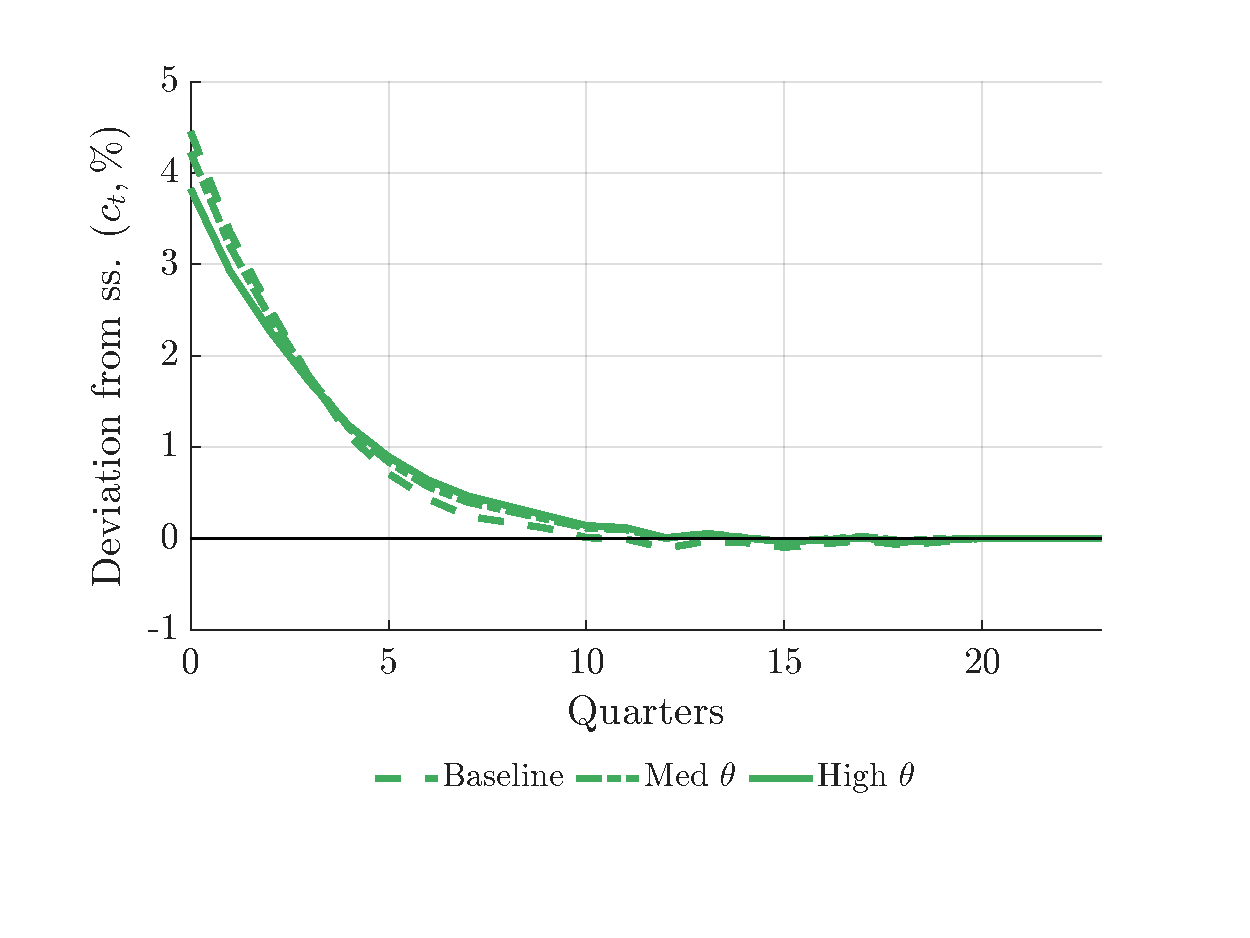
\includegraphics[width=\linewidth]{../../pro-default-model/results/comparison_figure_19.pdf}\\[-0.5em]
    {\scriptsize Consumption}
    \column{0.5\textwidth}
    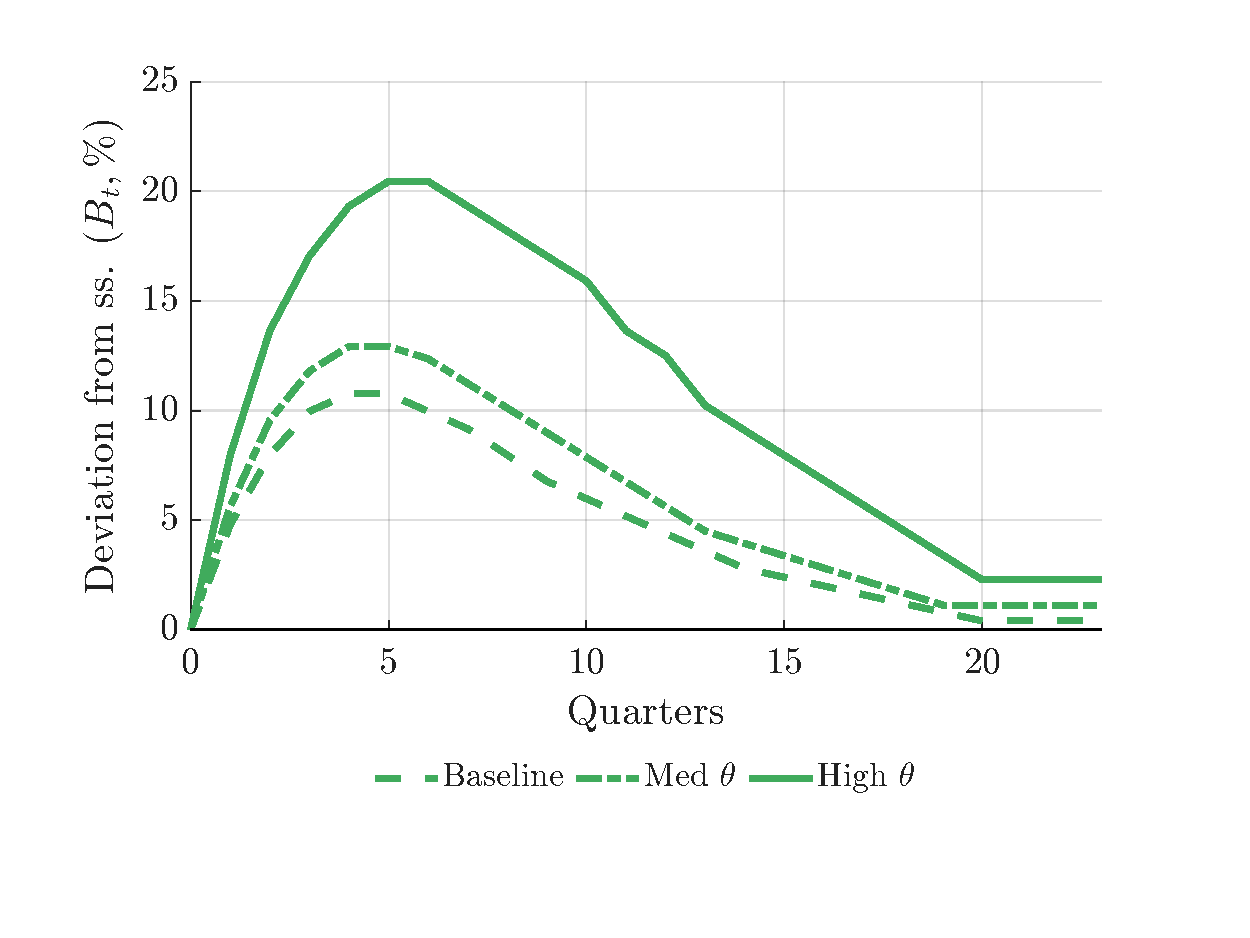
\includegraphics[width=\linewidth]{../../pro-default-model/results/comparison_figure_18.pdf}\\[-0.5em]
    {\scriptsize Debt}
    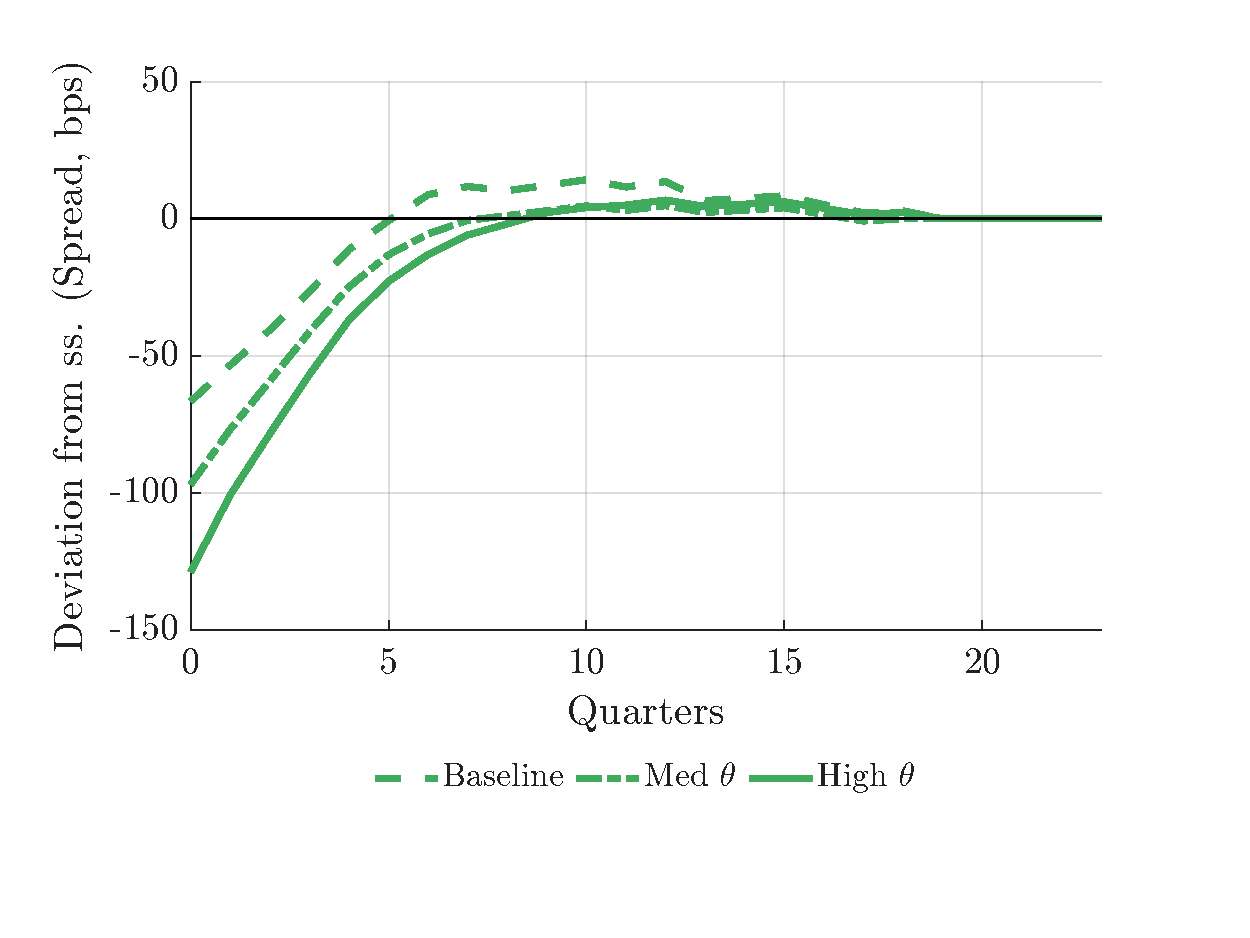
\includegraphics[width=\linewidth]{../../pro-default-model/results/comparison_figure_20.pdf}\\[-0.5em]
    {\scriptsize Spread}
  \end{columns}
\end{frame}

% Microfoundation
\section{Microfoundation (RI)}

\begin{frame}{Rational Inattention: Tail Weight from Attention}
  \begin{itemize}
    \item Lenders choose \textbf{precisions} $(a_\mu,a_\sigma)$ at convex cost
          $\Phi(a_\mu,a_\sigma)$.
    \item \textbf{FOC}: $\varphi\,\mathcal S=\kappa_\sigma a_\sigma\Rightarrow a_\sigma=\tfrac{\varphi}{\kappa_\sigma}\,\mathcal S$.
    \item \textbf{Tail weight}: $\displaystyle \theta_{\mathrm{RI}}(y,B')=\min\Big\{\,1+\frac{\varphi^2}{\kappa_\sigma}\,\mathcal S(y,B')\,,\;\bar\theta\,\Big\}$.
    \item Pricing remains the \textbf{same operator} at $\theta_{\mathrm{RI}}(\cdot)$;
          comparative statics \textbf{inherit}.
  \end{itemize}
  \vspace{0.5em}
  \begin{equation*}
    q(B',y)=\mathcal T_{\theta_{\mathrm{RI}}(y,B')}[q](B',y),\qquad \mathcal S=\E\Big[\partial U/\partial\theta\Big]\ge0.
  \end{equation*}
\end{frame}

\begin{frame}{Empirical Hook: Misreporting \texorpdfstring{$\Rightarrow$}{=>} Higher Dispersion Attention}
  \begin{itemize}
    \item \textbf{Degraded mean-information} ($a_\mu$) raises marginal value of dispersion info $\mathcal S$.
    \item $\uparrow\mathcal S\Rightarrow \uparrow a_\sigma\Rightarrow \uparrow \theta_{\mathrm{RI}}$: \textbf{higher average spreads}, \textbf{steeper pivot}, \textbf{decoupling}.
  \end{itemize}
\end{frame}

% Policy and information
\section{Policy \& Information}

\begin{frame}{Ramsey with PRO: Transfers Cannot Undo Price Wedge}
  \begin{gather*}
    c_t+\kappa B_t+\tau_t = y_t+\big(B_{t+1}-(1{-}\delta)B_t\big)\,q_{\theta}(y_t,B_{t+1}),\\
    \E_0\sum_t \beta^t\tau_t=0,\quad u'(\cdot)>0,\ u''(\cdot)<0.
  \end{gather*}
  \begin{itemize}
    \item \textbf{Intertemporal trade price} distorted by PRO persists in implementability; \textbf{deadweight loss}.
    \item \textbf{Result}: $W^R_{\theta}<W^R_1$ even with optimal transfers.
  \end{itemize}
\end{frame}

\begin{frame}{Endogenous Beliefs and Transparency}
  Belief dynamics with negativity bias:
  \begin{gather*}
    \theta_{t+1}=\lambda\,\theta_t+(1{-}\lambda)\,\widehat\theta(\{d_s\}),\quad
    \xi(y,B)=\max\Big\{0,\tfrac{P_1-P_{\theta_t}}{P_1}\Big\},\quad \text{defaults move beliefs more}.
  \end{gather*}
  Effective transparency:
  \begin{gather*}
    \theta_{\mathrm{eff}}(\alpha,\theta)=\alpha\cdot 1+(1{-}\alpha)\cdot\theta,\qquad
    \alpha^*:\ \frac{\mathrm d}{\mathrm d\alpha}W(\alpha)=\gamma\alpha.
  \end{gather*}
  \begin{itemize}
    \item \textbf{Persistent PRO} in invariant beliefs; \textbf{optimal transparency rises} with PRO severity.
  \end{itemize}
\end{frame}

% Computation
\section{Computation}

\begin{frame}{Computation and Stability}
  \begin{itemize}
    \item \textbf{Value and price iteration} on $(N_y{=}201, N_B{=}600)$ grid; OpenMP parallel.
    \item \textbf{Stabilized log-sum-exp} for borrowing/default logits; \textbf{infeasible-consumption guard}.
    \item \textbf{Convergence} tolerances $10^{-6}$; long simulation for moments and IRFs.
  \end{itemize}
  \vspace{0.5em}
  \centering
  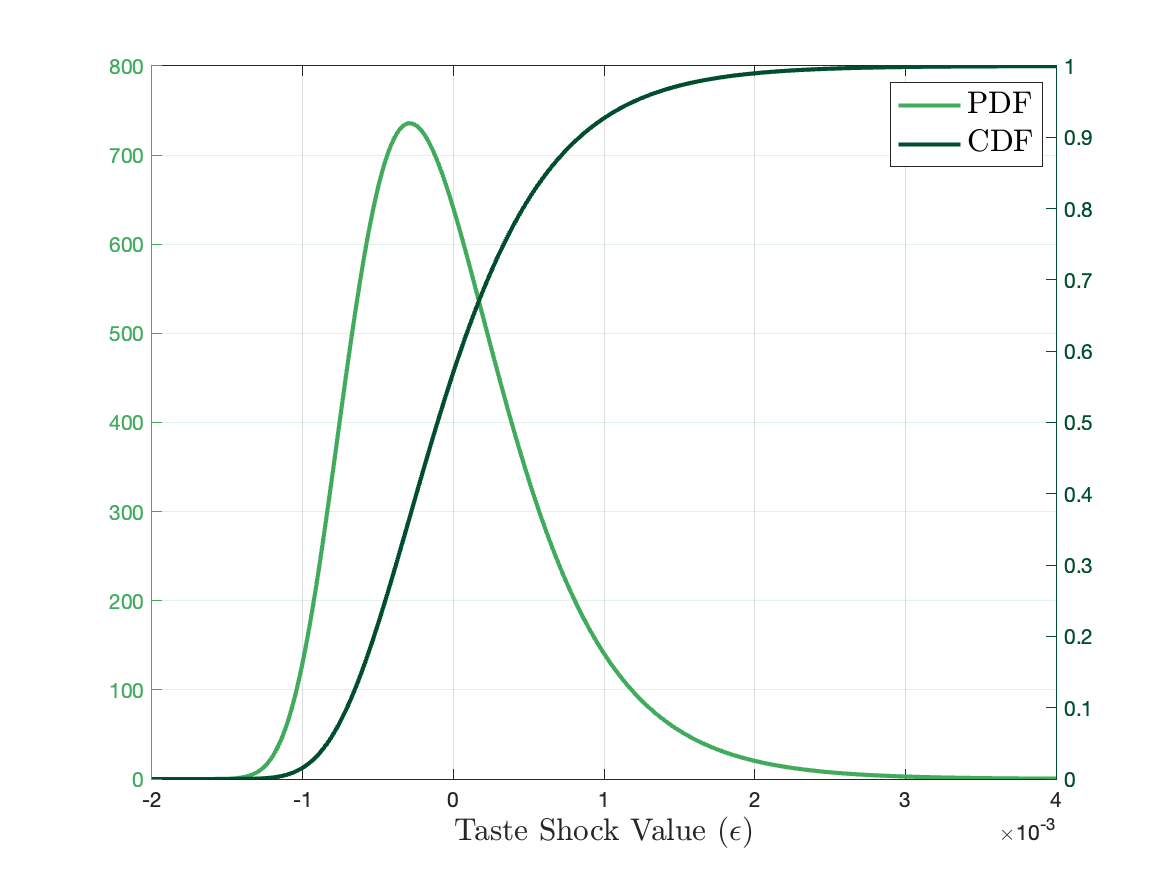
\includegraphics[width=0.6\linewidth]{../../paper/Long_term/gumbel_distribution.png}
  \\
  {\scriptsize Mean-zero Gumbel: \textbf{logit and LSE} arise naturally}
\end{frame}

% Conclusion
\section{Conclusion}

\begin{frame}{Takeaways}
  \begin{itemize}
    \item \textbf{Single operator + PRO} $\Rightarrow$ \textbf{pivot} in price/spread schedules.
    \item \textbf{Deleveraging} yet \textbf{higher average spreads}; volatility \textbf{falls} (\textbf{stability illusion}).
    \item \textbf{RI microfoundation} endogenizes tail tilt; \textbf{policy/info} extensions clarify limits and levers.
    \item Event hooks (Argentina) align with \textbf{pivot}, \textbf{threshold}, and
          \textbf{decoupling} predictions.
  \end{itemize}
\end{frame}

% Literature Review
\section{Literature Review}

\begin{frame}{Sovereign Default: Canonical and Extensions}
  \begin{itemize}
    \item \textbf{Canonical strategic default}: Eaton\,–\,Gersovitz (1981); Aguiar\,–\,Gopinath (2007); Arellano (2008);
          long-term debt: Hatchondo\,–\,Martinez (2009); Chatterjee\,–\,Eyigungor (2012); Mendoza\,–\,Yue (2012).
    \item \textbf{Empirics}: Tomz\,–\,Wright (2013); Meyer\,–\,Reinhart\,–\,Trebesch (2022); event studies (Argentina misreporting).
    \item \textbf{Reputation}: Cole\,–\,Dow\,–\,English (1995); Phelan (2006); Amador\,–\,Phelan (2021, 2023);
          learning via policy signals (Fourakis, 2024).
  \end{itemize}
\end{frame}

\begin{frame}{Beliefs, Ambiguity, and Information}
  \begin{itemize}
    \item \textbf{Ambiguity/robust control}: Hansen\,–\,Sargent (2001, 2008);
          smooth/variational prefs (Klibanoff et al., 2005; Maccheroni et al., 2006);
          applications to default (Pouzo\,–\,Presno, 2016; Roch\,–\,Roldan, 2023).
    \item \textbf{Behavioral beliefs}: Diagnostic expectations (Gennaioli\,–\,Shleifer, 2018; Bordalo et al., 2023);
          sentiment, noise trading, limits to arbitrage.
    \item \textbf{Information choice}: Rational inattention (Sims, 2003; Mačkowiak\,–\,Wiederholt, 2009; Matejka\,–\,McKay, 2015);
          macro finance (Veldkamp, 2011).
  \end{itemize}
  \vspace{0.3em}
  \textbf{This paper}: \emph{second-moment} belief wedge (PRO) \Rightarrow \textbf{pivot}, \textbf{deleveraging}, \textbf{stability illusion};
  RI microfoundation embeds \textbf{in the same operator}.
\end{frame}

% Deeper Math Details
\section{Deeper Math}

\begin{frame}{Bellman Aggregator and Sensitivities}
  \begin{gather*}
    J_\rho[V](y,B)=\rho\ln\sum_{B'}\exp\tfrac{W(y,B,B')}{\rho},\quad V(y,B)=\eta\ln\Big(e^{V^D/\eta}+e^{V^R/\eta}\Big).\\
    \frac{\partial V}{\partial q}\;=\;u'(c)\,\big[B'-(1{-}\delta)B\big]\cdot \text{softmax}(W/\rho).\quad (\text{Envelope over } B')
  \end{gather*}
  \begin{itemize}
    \item Lipschitz: $\|J(V_1){-}J(V_2)\|\le\beta\|V_1{-}V_2\|$,
          $\|J(\cdot,q_1){-}J(\cdot,q_2)\|\le L_{Jq}\|q_1{-}q_2\|$.
    \item Pricing: $\|T(V_1,\cdot){-}T(V_2,\cdot)\|\le L_{TV}\|V_1{-}V_2\|$,
          $\|T(\cdot,q_1){-}T(\cdot,q_2)\|\le m_q\|q_1{-}q_2\|$.
    \item \textbf{Slope condition}: $L_{Jq}L_{TV}<(1-\beta)(1-m_q)$ with $m_q=(1-\delta)/(1+r)$.
  \end{itemize}
\end{frame}

\begin{frame}{From $\partial_{\theta} P$ to $\partial_{\theta} q$}
  \begin{gather*}
    P_{\theta}=\Lsig\!\Big(-\tfrac{\Delta V}{\theta\eta}\Big),\quad \partial_{\theta} P_{\theta}\;=\;L'(\cdot)\,\tfrac{\Delta V}{\theta^2\eta}.\\
    (I-\mathcal T_{\theta})'\,\partial_{\theta} q_{\theta}\;=\;\partial_{\theta} \mathcal T_{\theta}[q_{\theta}],\quad (I-\mathcal T_{\theta})^{-1}\ge0.\\
    \Rightarrow\ \mathrm{sign}(\partial_{\theta} q_{\theta}) \text{ follows from } \mathrm{sign}(\partial_{\theta} P_{\theta}) \text{ and positivity of }(I{-}\mathcal T_{\theta})^{-1}.
  \end{gather*}
  \textbf{Implication}: \textbf{pivot} persists under smooth perturbations and state-dependent $\theta_{\mathrm{RI}}(y,B')$.
\end{frame}

% Backup (optional)
\appendix
\section{Backup}

\begin{frame}{Operator View (Sketch)}
  \begin{itemize}
    \item $\mathcal T_{\theta}$ is positive and order-preserving; fixed point unique under slope condition.
    \item Fixed-point differentiation signs $\partial_{\theta} q_{\theta}$; monotone
          propagation yields pivot.
  \end{itemize}
\end{frame}

\end{document}
